% SETUP DOCUMENTO %
\documentclass[onecolumn]{article}
\usepackage[italian]{babel}

\usepackage{tgschola}
\linespread{1.25}
\usepackage[fontsize=12pt]{scrextend}
\usepackage[a4paper,top=2.5cm,bottom=2.5cm,left=3cm,right=3cm,marginparwidth=1.75cm,footskip=1.5cm,heightrounded]{geometry}

\usepackage{subfig}
\usepackage{xcolor}
\definecolor{linkColor}{RGB}{2,11,120}
\definecolor{bgTitleRed}{RGB}{85,45,50}

% STILE BLOCCHI DI CODICE %
\usepackage[T1]{fontenc}
\usepackage[ttdefault=true]{AnonymousPro}
\usepackage{listings}
\usepackage{minted}
\usepackage{tcolorbox}
\tcbuselibrary{listings, breakable, minted, skins}
\tcbset{listing engine=minted}

\newtcblisting{bashCode}[2][]{
    breakable,
    listing only, #1 ,title=#2,
    minted language=bash,
    minted style=vs,
    coltitle=white,
    colbacktitle=bgTitleRed,
    toptitle=3mm, bottomtitle=2.5mm,
    top=2mm, bottom=3mm,
    fonttitle=\ttfamily,
    enhanced, frame hidden, 
    minted options={fontfamily=AnonymousPro, 
    tabsize=4, breaklines, autogobble, linenos=false}}

\setminted[python]{fontfamily=AnonymousPro, fontsize=\footnotesize, breaksymbol=.}

\usepackage[colorlinks=true, allcolors=linkColor]{hyperref}
\newcommand\anchor[2]{%
  \href{#2}{#1}\footnote{\url{#2}}%
}
\usepackage{graphicx}
\usepackage{amsmath}
\usepackage{float}

\usepackage{subfig}
\graphicspath{ {./images/} }

% INTESTAZIONE %
\title{Relazione Laboratorio Algoritmi\\\textit{Esercizio B}}
\author{Alberto Del Buono Paolini}
\date{Ottobre 2023}

\begin{document}
\begin{onecolumn}
\vspace*{-4em}
{\let\newpage\relax\maketitle}
\tableofcontents
\end{onecolumn}
\vspace{1cm}
\pagebreak

% CONTENUTO %
\section{Descrizione del problema}

\subsection{Introduzione}
Questa relazione mira ad analizzare e commentare il calcolo delle statistiche d'ordine dinamiche \textit{os-select} e \textit{os-rank}, mettendo a confronto le seguenti strutture dati: 
\begin{enumerate}
\setlength\itemsep{-0.25em}
    \item Lista ordinata
    \item Albero binario di ricerca senza attributo \textit{size}
    \item Albero rosso-nero con attributo \textit{size}
\end{enumerate}

L'obiettivo è valutare le prestazioni e le caratteristiche di ciascuna implementazione attraverso test ed esperimenti pratici, confrontandole con le evidenze teoriche descritte in questo capitolo.

\subsection{Caratteristiche teoriche}

Per prima cosa dobbiamo descrivere la natura di queste tre strutture dati e delle statistiche d'ordine dinamiche che andremo ad analizzare. Esamineremo quindi nei vari casi le complessità computazionali di:

\begin{enumerate}
\setlength\itemsep{-0.25em}
    \item \textit{os-select(k)}: è un'operazione che trova l'elemento con un rango specifico $k$ in un insieme di dati, cioè restituisce il $k$-esimo elemento più piccolo dell'insieme di dati.
    \item \textit{os-rank(x)}: è un'operazione che calcola il rango di un elemento specifico $x$ all'interno di un insieme di dati, dove il rango di un elemento è il numero di elementi nell'insieme che sono inferiori o uguali a $x$.
\end{enumerate}

\subsubsection{Lista collegata ordinata}

Questa è una struttura composta da nodi che hanno attributi \textit{value} (il valore del dato contenuto nel nodo) e \textit{next} (un puntatore al nodo successivo della lista oppure vuoto). Per attraversare completamente una lista collegata con puntatori bisogna quindi partire dal primo nodo (chiamato solitamente \textit{head}) e spostarsi sui nodi successivi tramite il puntatore \textit{next}, fino a che non è vuoto, a significare la fine della lista. Inoltre è una struttura ordinata: ogni nodo viene inserito nella lista in base al valore del suo dato (con ordine ascendente o discendente). Supponiamo di essere nel caso di ordine ascendente, come mostrato in \hyperref[fig:lista]{figura 1}.

\begin{figure}
  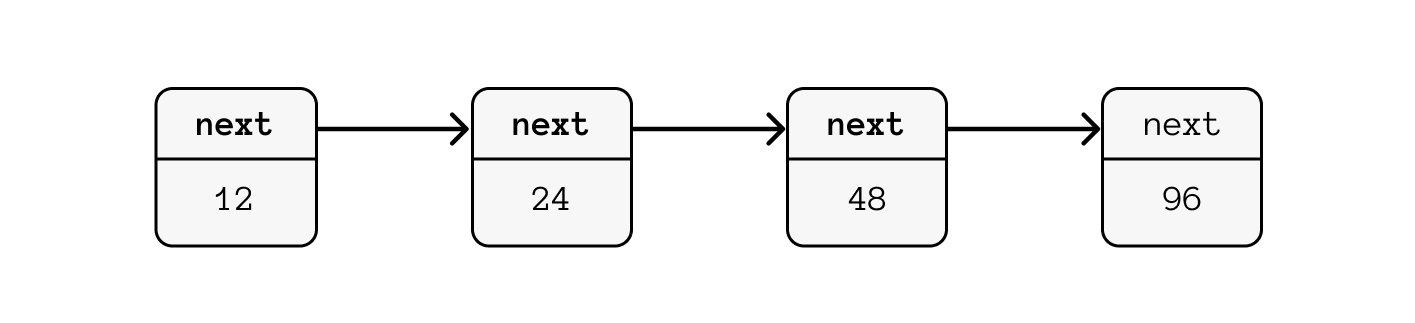
\includegraphics[width=\linewidth]{lista.png}
  \caption{Lista collegata con puntatori}
  \label{fig:lista}
\end{figure}

\textbf{os-select}: questa operazione richiede di scorrere la lista dall'inizio, contando gli elementi fino a raggiungere il $k$-esimo. Questo significa che il tempo necessario per trovare questo elemento cresce linearmente con $k$ e, nel caso peggiore, bisognerà scorrere tutta la lista lunga $n$. La complessità di os-select è quindi $O(k)$ e $\Theta(n)$ nel caso peggiore. \vspace{0.5em}

\textbf{os-rank}: Per determinare il rango di un elemento x bisogna scorrere la lista contando quante chiavi sono inferiori a $x$, perciò le complessità sono uguali a os-select. La lista collegata ordinata non è molto efficiente per il calcolo delle due statistiche d'ordine, specialmente quando si cerca un $k$ o un $x$ grande. 

\subsubsection{Albero binario di ricerca}

Un albero binario di ricerca è una struttura dati gerarchica composta da nodi collegati tra loro. Ogni nodo ha attributi per al massimo due figli, uno a sinistra (\textit{left}) e uno a destra (\textit{right}), e un valore (\textit{value}) che soddisfi le seguenti proprietà:

\begin{enumerate}
\setlength\itemsep{-0.25em}
    \item I valori nei nodi del sottoalbero sinistro sono inferiori o uguali al valore nel nodo padre.
    \item I valori nei nodi del sottoalbero destro sono superiori al valore nel nodo padre.
\end{enumerate}

Quindi per qualsiasi nodo nell'ABR (illustrato in \hyperref[fig:alberi]{figura 2a}), tutti i nodi nei sottoalberi a sinistra contengono valori inferiori o uguali, e tutti i nodi nei sottoalberi a destra contengono valori superiori; questo aiuta la complessità del calcolo delle statistiche d'ordine. \vspace{1em}

\textbf{os-select}: Questo metodo attraversa un singolo percorso nell'albero per trovare il $k$-esimo elemento e la complessità è $O(h)$, dove $h$ è l'altezza dell'albero. Il tempo di esecuzione dipende dall'altezza dell'albero e dalla struttura specifica dell'albero. Se l'albero è bilanciato, l'altezza è $\Theta(\log n)$, garantendo una complessità di $O(\log n)$ nel caso peggiore. \vspace{0.5em}

\textbf{os-rank}: anche os-rank richiede un percorso nell'albero fino a un elemento specifico $x$ e ha una complessità temporale di $O(h)$. Sarebbe necessaria la costante riequilibratura dell'albero per mantenere la complessità $O(\log n)$. Tuttavia, se l'albero è sbilanciato con un unico ramo, la complessità può arrivare fino a $\Theta(n)$, ugualmente ad os-select.

\begin{figure}
  \centering
    \subfloat[Albero binario di ricerca]{{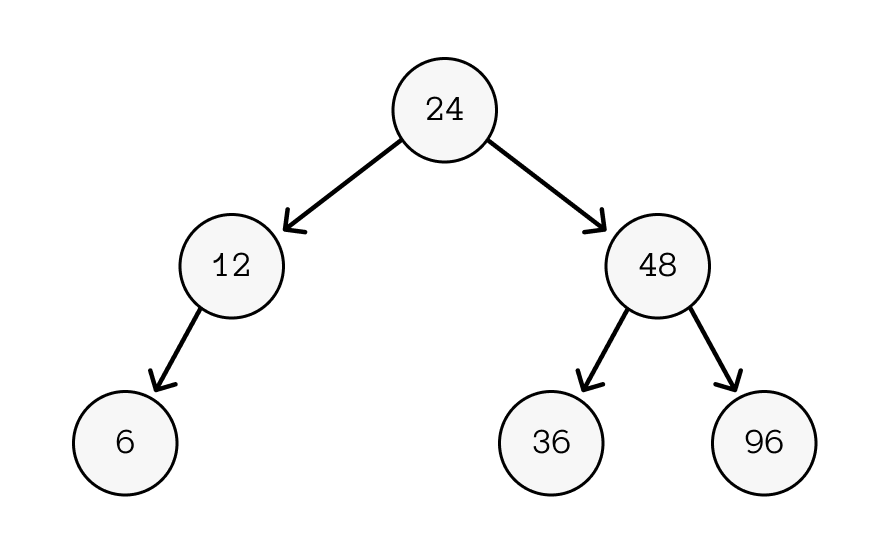
\includegraphics[width=\linewidth/2-1.5em]{abr} }}
    \qquad
    \subfloat[Albero rosso-nero aumentato]{{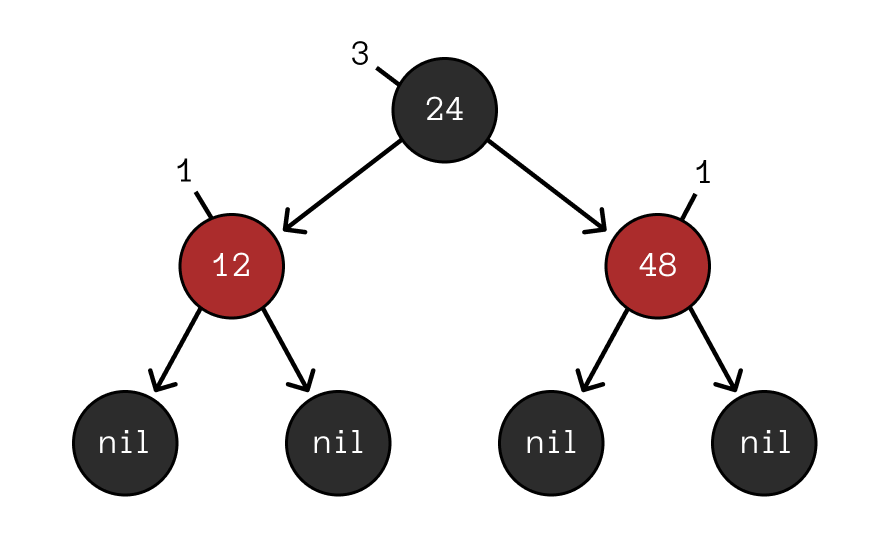
\includegraphics[width=\linewidth/2-1.5em]{arn} }}
    \caption{Illustrazioni alberi}
    \label{fig:alberi}
\end{figure}

\subsubsection{Albero rosso-nero aumentato con attributo \textit{size}}

Gli alberi rosso-neri aumentati sono una variante dei tradizionali alberi rosso-neri. Le proprietà di un albero rosso-nero sono estese da quelle di un albero binario di ricerca con la seguente: ogni nodo in un ARN è etichettato come \textit{rosso} o \textit{nero} nell'attributo \textit{color}, seguendo le seguenti regole per garantire che l'albero sia bilanciato:

\begin{enumerate}
\setlength\itemsep{-0.25em}
    \item Un nodo è o rosso o nero.
    \item La radice dell'albero è nera.
    \item Non possono esistere due nodi rossi consecutivi lungo qualsiasi cammino dall'alto verso il basso.
\end{enumerate}

Gli ARN aumentati (in \hyperref[fig:alberi]{figura 2b}) includono una modifica aggiuntiva: l'attributo \textit{size} in ciascun nodo dell'albero. Questo attributo tiene traccia del numero di nodi nel sottoalbero con radice in quel nodo (include anche il nodo stesso) e velocizza in media il calcolo del rango di un elemento all'interno dell'albero. \vspace{1em}

\textbf{os-select}: l'operazione di os-select è molto efficiente grazie all'attributo \textit{size}, possiamo trovare il $k$-esimo elemento sempre in $O(h)$ e $\Theta(\log n)$ nel caso peggiore. \vspace{0.5em}

\textbf{os-rank}: Anche l'operazione di os-rank ha una complessità di $O(h)$ e di $\Theta(\log n)$ nel caso peggiore. \vspace{1em}

In generale, l'implementazione con l'albero rosso-nero aumentato con l'attributo \textit{size} eccelle in entrambe le statistiche, offrendo prestazioni notevolmente migliori rispetto alla lista collegata ordinata e agli ABR non bilanciati, essendo gli ARN bilanciati ad ogni inserimento.

\section{Descrizione degli esperimenti}
\subsection{Piattaforma di esecuzione}

Per sviluppare il codice ed eseguire tutti i test, ottenendo le tabelle e i grafici riportati in questo documento, è stata utilizzata un'istanza di \anchor{Gitpod}{https://www.gitpod.io/} con le seguenti specifiche:
\begin{bashCode}{Output neofetch}
OS: Ubuntu 22.04.3 LTS x86_64 
Host: Google Compute Engine 
Kernel: 6.1.54-060154-generic 
CPU: AMD EPYC 7B13 (16 cores) @ 2.449GHz 
Memory: 30099MiB / 64297MiB
\end{bashCode}

\subsection{Strategia di iterazione}

\textbf{Iterazione casuale}: Esegui le operazioni in modo casuale sugli elementi dell'insieme di dati. Questo è utile per valutare le prestazioni in scenari realistici in cui le operazioni potrebbero essere distribuite in modo casuale nel tempo.

\subsection{Dimensioni delle strutture dati}

Esegui i tuoi test su diverse dimensioni delle strutture dati per valutare come le prestazioni variano con l'aumento del numero di elementi nell'insieme di dati. Ad esempio, puoi testare le prestazioni su insiemi di dati di dimensioni 10, 100, 1000, ecc.

Assicurati di considerare sia casi di piccole dimensioni che casi di grandi dimensioni, poiché le prestazioni possono differire notevolmente in base alle dimensioni dell'insieme di dati.

\subsection{Ripetizioni dei test}

Per ottenere risultati affidabili, esegui ciascun test più volte e calcola la media dei tempi di esecuzione. Questo ridurrà l'impatto di variazioni casuali e fornirà risultati più stabili.

Puoi anche calcolare la deviazione standard o l'intervallo di confidenza per misurare la variabilità dei risultati.

\subsection{Randomizzazione}

L'uso di dati casuali durante i test può essere utile per valutare le prestazioni in scenari realistici.

\newpage
\section{Documentazione del codice}

La struttura delle classi è osservabile nel diagramma UML in \hyperref[fig:classi]{figura 3}; segue una breve descrizione di ogni attributo e metodo implementato per eseguire i test sulle statistiche d'ordine dinamiche. 

\begin{figure}[h!]
  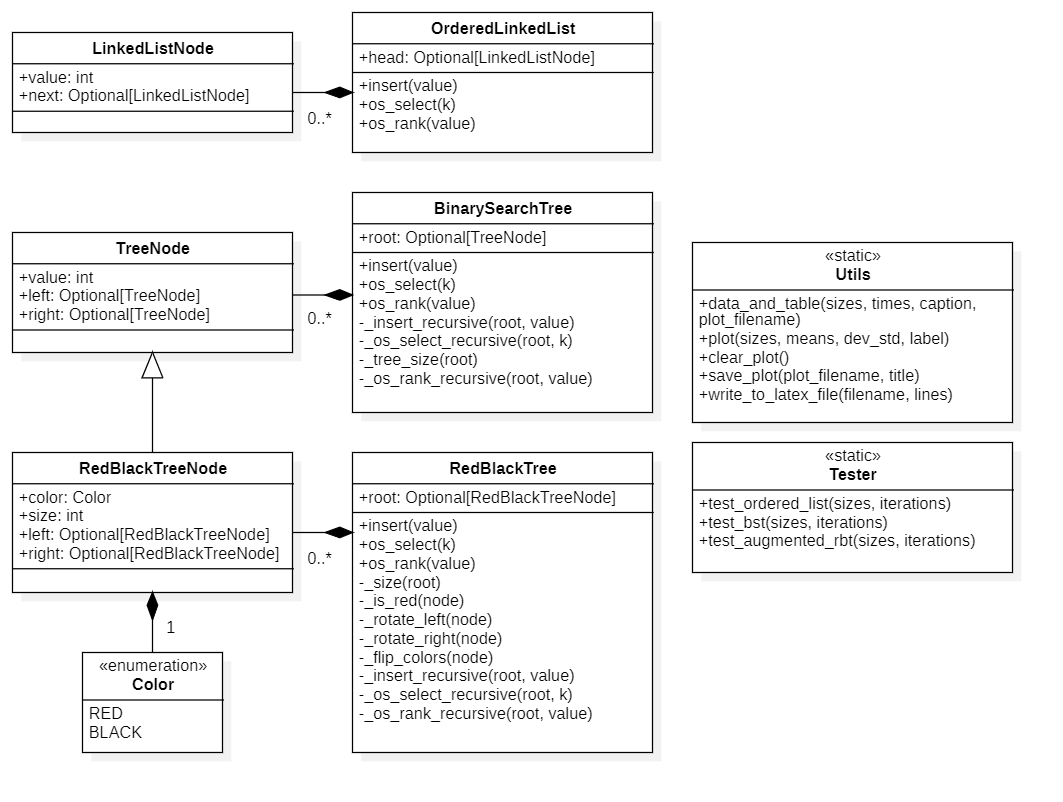
\includegraphics[width=\linewidth]{classi.png}
  \caption{Diagramma UML delle classi}
  \label{fig:classi}
\end{figure}

\subsection{Lista collegata ordinata}
\texttt{\textbf{LinkedListNode}}
\begin{itemize}
\setlength\itemsep{0em}
    \item \verb|value|: il valore memorizzato nel nodo
    \item \verb|next|: il riferimento al nodo successivo
\end{itemize}

{\setlength{\parindent}{0em} \texttt{\textbf{OrderedLinkedList}}}
\begin{itemize}
\setlength\itemsep{0em}
    \item \verb|head|: il riferimento al primo nodo nella lista (di tipo \texttt{LinkedListNode})
    \item \verb|insert(value)|: inserisce un nuovo nodo con il valore specificato nella lista in modo ordinato
    \item \verb|os_select(k)|: restituisce il valore dell'elemento con rango $k$ nella lista
    \item \verb|os_rank(value)|: restituisce il rango dell'elemento con valore specificato nella lista
\end{itemize}

\subsection{Albero binario di ricerca}
\texttt{\textbf{TreeNode}}
\begin{itemize}
\setlength\itemsep{0em}
    \item \verb|value|: il valore memorizzato nel nodo
    \item \verb|left|: il riferimento al figlio sinistro
    \item \verb|right|: il riferimento al figlio destro
\end{itemize}

{\setlength{\parindent}{0em} \texttt{\textbf{BinarySearchTree}}}
\begin{itemize}
\setlength\itemsep{0em}
    \item \verb|root|: il riferimento alla radice dell'albero (di tipo \texttt{TreeNode})
    \item \verb|insert(value)|: inserisce un nuovo nodo con il valore specificato nell'albero binario di ricerca
    \item \verb|os_select(k)|: restituisce il valore dell'elemento con rango $k$ nell'albero binario di ricerca
    \item \verb|_tree_size(root)|: calcola la dimensione (numero di nodi) del sottoalbero radicato in un nodo specifico
    \item \verb|os_rank(value)|: restituisce il rango dell'elemento con valore specificato nell'albero binario di ricerca
\end{itemize}

\subsection{Albero rosso-nero aumentato con attributo \textit{size}}
\texttt{\textbf{RedBlackTreeNode}}
\begin{itemize}
\setlength\itemsep{0em}
    \item \verb|color|: il colore del nodo (ROSSO o NERO)
    \item \verb|size|: il numero di nodi nel sottoalbero radicato in questo nodo
    \item \verb|left|: il riferimento al figlio sinistro
    \item \verb|right|: il riferimento al figlio destro
    \item \verb|value|: il valore memorizzato nel nodo (ereditato dalla classe \texttt{TreeNode})
\end{itemize}

{\setlength{\parindent}{0em} \texttt{\textbf{AugmentedRedBlackTree}}}
\begin{itemize}
\setlength\itemsep{0em}
    \item \verb|root|: il riferimento alla radice dell'albero rosso-nero aumentato (di tipo \texttt{RedBlackTreeNode})
    \item \verb|insert(value)|: inserisce un nuovo nodo con il valore specificato nell'albero rosso-nero aumentato
    \item \verb|os_select(k)|: restituisce il valore dell'elemento con rango $k$ nell'albero rosso-nero aumentato
    \item \verb|os_rank(value)|: restituisce il rango dell'elemento con valore specificato nell'albero rosso-nero aumentato
    \item \verb|_size(root)|: calcola la dimensione (numero di nodi) del sottoalbero radicato in un nodo specifico
    \item \verb|_is_red(node)|: verifica se il nodo specificato è di colore ROSSO
    \item \verb|_rotate_left(g)|: esegue una rotazione sinistra nell'albero rosso-nero
    \item \verb|_rotate_rigth(g)|: esegue una rotazione destra nell'albero rosso-nero
    \item \verb|_flip_colors(g)|: inverte i colori dei nodi nell'albero rosso-nero
\end{itemize}

\subsection{Classi \texttt{Tester} e \texttt{Utils}}
\texttt{\textbf{Tester}}
\begin{itemize}
\setlength\itemsep{0em}
    \item \verb|test_ordered_list(sizes, iterations)|: esegue test e raccolta dati per una lista collegata ordinata
    \item \verb|test_bst(sizes, iterations)|: esegue test e raccolta dati per un albero binario di ricerca
    \item \verb|test_augmented_rbt(sizes, iterations)|: esegue test e raccolta dati per un albero rosso-nero aumentato con attributo "size"
\end{itemize}

{\setlength{\parindent}{0em} \texttt{\textbf{Utils}}}
\begin{itemize}
\setlength\itemsep{0em}
    \item \verb|data_and_table(sizes, times, caption, plot_filename)|: genera dati e tabelle per le dimensioni specificate e i tempi di esecuzione
    \item \verb|plot(sizes, means, dev_std, label)|: crea un grafico con medie e deviazioni standard
    \item \verb|clear_plot()|: cancella il grafico corrente
    \item \verb|save_plot(plot_filename, title)|: salva il grafico corrente con un titolo specificato
    \item \verb|write_to_latex_file(filename, lines)|: scrive dati su file LaTeX con il nome specificato
\end{itemize}

\newpage
\section{Analisi dei risultati sperimentali}

In questa sezione, condurremo un'analisi completa dei risultati sperimentali. Discuteremo le discrepanze tra le prestazioni attese e quelle effettivamente osservate, se presenti, e offriremo interpretazioni basate sui dati raccolti. 

Riferimenti alle tabelle: \ref{Inserimento in una lista ordinata}, \ref{Rimozione in una lista ordinata}, \ref{Ricerca in una lista ordinata}, \ref{OS-Select in una lista ordinata}, \ref{OS-Rank in una lista ordinata}, \ref{Inserimento in un ABR}, \ref{Rimozione in un ABR}, \ref{Ricerca in un ABR}, \ref{OS-Select in un ABR}, \ref{OS-Rank in un ABR}, \ref{Inserimento in un albero RN aumentato}, \ref{Rimozione in un albero RN aumentato}, \ref{Ricerca in un albero RN aumentato}, \ref{OS-Select in un albero RN aumentato}, \ref{OS-Rank in un albero RN aumentato}.

\subsection{os-select}

\subsection{os-rank}

\section{Conclusioni}

Concluderemo la relazione con un riepilogo delle scoperte chiave e delle implicazioni dei risultati sperimentali. Discuteremo anche eventuali sviluppi futuri e possibili miglioramenti.

\newpage
\section{Tabelle}
\begin{table}
\centering
\caption{OS-Select in una lista ordinata}
\label{OS-Select in una lista ordinata}
\begin{adjustbox}{width=1\textwidth/2}
\begin{tabular}{|c|c|c|c|}
\hline
 & Dimensione (n) & Mediana (s) & Tempi -/+ (s) \\
0 & 10000 & 4.1e-04 & -4.1e-04, +9.7e-04 \\
\cline{1-4}
1 & 10500 & 4.6e-04 & -4.6e-04, +8.2e-04 \\
\cline{1-4}
2 & 11000 & 4.8e-04 & -4.8e-04, +2.2e-03 \\
\cline{1-4}
3 & 11500 & 5.0e-04 & -5.0e-04, +1.8e-03 \\
\cline{1-4}
4 & 12000 & 4.9e-04 & -4.9e-04, +9.2e-04 \\
\cline{1-4}
5 & 12500 & 5.9e-04 & -5.8e-04, +4.3e-03 \\
\cline{1-4}
6 & 13000 & 5.6e-04 & -5.6e-04, +3.7e-03 \\
\cline{1-4}
7 & 13500 & 5.8e-04 & -5.8e-04, +1.0e-03 \\
\cline{1-4}
8 & 14000 & 6.1e-04 & -6.1e-04, +1.1e-03 \\
\cline{1-4}
9 & 14500 & 6.3e-04 & -6.2e-04, +1.1e-03 \\
\cline{1-4}
10 & 15000 & 6.5e-04 & -6.5e-04, +3.7e-03 \\
\cline{1-4}
11 & 15500 & 6.7e-04 & -6.6e-04, +2.7e-03 \\
\cline{1-4}
12 & 16000 & 7.1e-04 & -7.1e-04, +2.7e-03 \\
\cline{1-4}
13 & 16500 & 7.1e-04 & -7.1e-04, +3.0e-03 \\
\cline{1-4}
14 & 17000 & 7.4e-04 & -7.4e-04, +3.6e-03 \\
\cline{1-4}
15 & 17500 & 7.8e-04 & -7.8e-04, +2.3e-03 \\
\cline{1-4}
16 & 18000 & 8.6e-04 & -8.6e-04, +3.3e-03 \\
\cline{1-4}
17 & 18500 & 8.6e-04 & -8.6e-04, +5.4e-03 \\
\cline{1-4}
18 & 19000 & 8.2e-04 & -8.2e-04, +1.9e-03 \\
\cline{1-4}
19 & 19500 & 9.3e-04 & -9.3e-04, +8.2e-03 \\
\cline{1-4}
20 & 20000 & 9.3e-04 & -9.3e-04, +5.5e-03 \\
\cline{1-4}
\end{tabular}
\end{adjustbox}
\end{table}

\begin{table}
\centering
\caption{OS-Rank in una lista ordinata}
\label{OS-Rank in una lista ordinata}
\begin{adjustbox}{width=1\textwidth/2}
\begin{tabular}{|c|c|c|c|}
\hline
 & Dimensione (n) & Mediana (s) & Tempi -/+ (s) \\
0 & 10000 & 4.7e-04 & -4.7e-04, +1.4e-03 \\
\cline{1-4}
1 & 10500 & 5.1e-04 & -5.1e-04, +9.3e-04 \\
\cline{1-4}
2 & 11000 & 5.7e-04 & -5.7e-04, +3.2e-03 \\
\cline{1-4}
3 & 11500 & 5.8e-04 & -5.8e-04, +4.6e-03 \\
\cline{1-4}
4 & 12000 & 5.5e-04 & -5.4e-04, +3.2e-03 \\
\cline{1-4}
5 & 12500 & 6.4e-04 & -6.3e-04, +5.5e-03 \\
\cline{1-4}
6 & 13000 & 6.3e-04 & -6.3e-04, +2.1e-03 \\
\cline{1-4}
7 & 13500 & 6.6e-04 & -6.6e-04, +4.2e-03 \\
\cline{1-4}
8 & 14000 & 7.3e-04 & -7.3e-04, +1.3e-03 \\
\cline{1-4}
9 & 14500 & 7.1e-04 & -7.1e-04, +1.4e-03 \\
\cline{1-4}
10 & 15000 & 8.0e-04 & -8.0e-04, +6.2e-03 \\
\cline{1-4}
11 & 15500 & 8.0e-04 & -8.0e-04, +1.8e-03 \\
\cline{1-4}
12 & 16000 & 8.3e-04 & -8.3e-04, +2.7e-03 \\
\cline{1-4}
13 & 16500 & 8.1e-04 & -8.1e-04, +3.0e-03 \\
\cline{1-4}
14 & 17000 & 8.9e-04 & -8.9e-04, +8.4e-03 \\
\cline{1-4}
15 & 17500 & 8.2e-04 & -8.1e-04, +4.2e-03 \\
\cline{1-4}
16 & 18000 & 1.0e-03 & -1.0e-03, +7.1e-03 \\
\cline{1-4}
17 & 18500 & 9.1e-04 & -9.1e-04, +3.7e-03 \\
\cline{1-4}
18 & 19000 & 9.8e-04 & -9.7e-04, +4.6e-03 \\
\cline{1-4}
19 & 19500 & 1.2e-03 & -1.2e-03, +1.3e-02 \\
\cline{1-4}
20 & 20000 & 1.1e-03 & -1.1e-03, +4.3e-03 \\
\cline{1-4}
\end{tabular}
\end{adjustbox}
\end{table}

\begin{table}
\centering
\caption{OS-Select in un ABR}
\label{OS-Select in un ABR}
\begin{adjustbox}{width=1\textwidth/2}
\begin{tabular}{|c|c|c|c|}
\hline
 & Dimensione (n) & Mediana (s) & Tempi -/+ (s) \\
0 & 10 & 1.4e-06 & -5.3e-07, +6.1e-06 \\
\cline{1-4}
1 & 20 & 2.6e-06 & -1.5e-06, +5.3e-06 \\
\cline{1-4}
2 & 30 & 4.0e-06 & -3.0e-06, +2.4e-05 \\
\cline{1-4}
3 & 40 & 4.1e-06 & -2.9e-06, +3.5e-05 \\
\cline{1-4}
4 & 50 & 8.9e-06 & -4.8e-06, +2.4e-05 \\
\cline{1-4}
5 & 60 & 1.0e-05 & -5.2e-06, +3.6e-05 \\
\cline{1-4}
6 & 70 & 8.3e-06 & -5.1e-06, +3.1e-05 \\
\cline{1-4}
7 & 80 & 1.1e-05 & -9.5e-06, +3.6e-05 \\
\cline{1-4}
8 & 90 & 1.4e-05 & -8.9e-06, +4.0e-02 \\
\cline{1-4}
9 & 100 & 1.9e-05 & -1.0e-05, +4.4e-05 \\
\cline{1-4}
10 & 110 & 1.2e-05 & -7.6e-06, +3.1e-05 \\
\cline{1-4}
11 & 120 & 2.1e-05 & -1.8e-05, +3.4e-05 \\
\cline{1-4}
12 & 130 & 3.1e-05 & -2.7e-05, +3.6e-05 \\
\cline{1-4}
13 & 140 & 2.3e-05 & -1.3e-05, +4.0e-05 \\
\cline{1-4}
14 & 150 & 2.8e-05 & -1.7e-05, +6.6e-05 \\
\cline{1-4}
15 & 160 & 2.4e-05 & -1.4e-05, +4.3e-05 \\
\cline{1-4}
16 & 170 & 3.2e-05 & -1.8e-05, +5.1e-05 \\
\cline{1-4}
17 & 180 & 3.1e-05 & -2.5e-05, +5.7e-05 \\
\cline{1-4}
18 & 190 & 4.3e-05 & -2.6e-05, +5.0e-05 \\
\cline{1-4}
19 & 200 & 2.0e-05 & -1.4e-05, +6.1e-05 \\
\cline{1-4}
20 & 210 & 4.1e-05 & -4.0e-05, +1.4e-04 \\
\cline{1-4}
21 & 220 & 2.8e-05 & -2.7e-05, +5.5e-05 \\
\cline{1-4}
22 & 230 & 4.5e-05 & -2.5e-05, +4.7e-05 \\
\cline{1-4}
23 & 240 & 2.5e-05 & -1.4e-05, +5.6e-05 \\
\cline{1-4}
24 & 250 & 3.8e-05 & -3.8e-05, +1.2e-02 \\
\cline{1-4}
25 & 260 & 2.0e-05 & -1.7e-05, +3.7e-05 \\
\cline{1-4}
26 & 270 & 4.3e-05 & -2.3e-05, +4.6e-05 \\
\cline{1-4}
27 & 280 & 4.8e-05 & -2.6e-05, +4.3e-05 \\
\cline{1-4}
28 & 290 & 6.3e-05 & -4.2e-05, +2.4e-04 \\
\cline{1-4}
29 & 300 & 7.8e-05 & -6.8e-05, +1.0e-04 \\
\cline{1-4}
30 & 310 & 2.9e-05 & -2.0e-05, +7.6e-05 \\
\cline{1-4}
31 & 320 & 3.2e-05 & -2.2e-05, +4.5e-05 \\
\cline{1-4}
32 & 330 & 5.4e-05 & -3.0e-05, +8.4e-05 \\
\cline{1-4}
33 & 340 & 5.0e-05 & -2.5e-05, +1.0e-04 \\
\cline{1-4}
34 & 350 & 3.3e-05 & -2.3e-05, +6.6e-05 \\
\cline{1-4}
35 & 360 & 3.4e-05 & -2.7e-05, +5.9e-05 \\
\cline{1-4}
36 & 370 & 5.3e-05 & -2.7e-05, +6.5e-05 \\
\cline{1-4}
37 & 380 & 5.6e-05 & -4.9e-05, +5.9e-05 \\
\cline{1-4}
38 & 390 & 1.1e-04 & -7.4e-05, +1.5e-04 \\
\cline{1-4}
39 & 400 & 7.8e-05 & -4.8e-05, +8.6e-05 \\
\cline{1-4}
\end{tabular}
\end{adjustbox}
\end{table}

\begin{table}
\centering
\begin{adjustbox}{width=1\textwidth/2}
\begin{tabular}{|c|c|c|c|}
\hline
 & Dimensione (n) & Mediana (s) & Tempi -/+ (s) \\
40 & 410 & 3.8e-05 & -2.1e-05, +6.3e-05 \\
\cline{1-4}
41 & 420 & 5.8e-05 & -3.7e-05, +6.8e-05 \\
\cline{1-4}
42 & 430 & 4.0e-05 & -3.2e-05, +9.7e-05 \\
\cline{1-4}
43 & 440 & 7.5e-05 & -6.3e-05, +1.1e-04 \\
\cline{1-4}
44 & 450 & 8.1e-05 & -5.1e-05, +9.1e-05 \\
\cline{1-4}
45 & 460 & 5.9e-05 & -4.8e-05, +1.1e-04 \\
\cline{1-4}
46 & 470 & 1.1e-04 & -6.7e-05, +9.8e-05 \\
\cline{1-4}
47 & 480 & 5.6e-05 & -4.7e-05, +8.2e-05 \\
\cline{1-4}
48 & 490 & 6.9e-05 & -4.0e-05, +8.8e-05 \\
\cline{1-4}
49 & 500 & 6.2e-05 & -3.2e-05, +7.2e-05 \\
\cline{1-4}
50 & 510 & 6.0e-05 & -4.0e-05, +2.1e-04 \\
\cline{1-4}
51 & 520 & 5.8e-05 & -3.9e-05, +6.1e-05 \\
\cline{1-4}
52 & 530 & 1.1e-04 & -7.0e-05, +1.5e-04 \\
\cline{1-4}
53 & 540 & 5.0e-05 & -2.9e-05, +1.3e-04 \\
\cline{1-4}
54 & 550 & 1.4e-04 & -8.9e-05, +1.4e-04 \\
\cline{1-4}
55 & 560 & 1.5e-04 & -9.8e-05, +3.5e-04 \\
\cline{1-4}
56 & 570 & 8.2e-05 & -3.9e-05, +8.2e-05 \\
\cline{1-4}
57 & 580 & 8.2e-05 & -4.1e-05, +1.3e-04 \\
\cline{1-4}
58 & 590 & 6.5e-05 & -4.9e-05, +2.6e-04 \\
\cline{1-4}
59 & 600 & 7.5e-05 & -4.9e-05, +8.9e-05 \\
\cline{1-4}
60 & 610 & 9.8e-05 & -9.3e-05, +9.9e-05 \\
\cline{1-4}
61 & 620 & 1.0e-04 & -6.3e-05, +1.0e-04 \\
\cline{1-4}
62 & 630 & 9.3e-05 & -5.7e-05, +1.3e-04 \\
\cline{1-4}
63 & 640 & 6.1e-05 & -2.8e-05, +7.5e-05 \\
\cline{1-4}
64 & 650 & 6.3e-05 & -5.1e-05, +8.9e-05 \\
\cline{1-4}
65 & 660 & 1.2e-04 & -7.6e-05, +3.1e-04 \\
\cline{1-4}
66 & 670 & 1.0e-04 & -6.0e-05, +1.5e-04 \\
\cline{1-4}
67 & 680 & 1.4e-04 & -7.8e-05, +2.3e-04 \\
\cline{1-4}
68 & 690 & 1.0e-04 & -6.1e-05, +8.3e-05 \\
\cline{1-4}
69 & 700 & 1.2e-04 & -6.6e-05, +1.4e-04 \\
\cline{1-4}
70 & 710 & 1.1e-04 & -5.3e-05, +1.9e-04 \\
\cline{1-4}
71 & 720 & 9.8e-05 & -9.5e-05, +1.2e-04 \\
\cline{1-4}
72 & 730 & 1.1e-04 & -6.2e-05, +1.9e-04 \\
\cline{1-4}
73 & 740 & 1.2e-04 & -6.9e-05, +5.6e-02 \\
\cline{1-4}
74 & 750 & 8.8e-05 & -8.0e-05, +1.6e-04 \\
\cline{1-4}
75 & 760 & 9.5e-05 & -5.1e-05, +1.1e-04 \\
\cline{1-4}
76 & 770 & 1.4e-04 & -7.3e-05, +1.8e-04 \\
\cline{1-4}
77 & 780 & 1.1e-04 & -9.0e-05, +2.0e-02 \\
\cline{1-4}
78 & 790 & 1.1e-04 & -9.0e-05, +2.1e-04 \\
\cline{1-4}
79 & 800 & 1.1e-04 & -7.4e-05, +2.6e-04 \\
\cline{1-4}
\end{tabular}
\end{adjustbox}
\end{table}

\begin{table}
\centering
\begin{adjustbox}{width=1\textwidth/2}
\begin{tabular}{|c|c|c|c|}
\hline
 & Dimensione (n) & Mediana (s) & Tempi -/+ (s) \\
80 & 810 & 7.8e-05 & -4.3e-05, +6.8e-05 \\
\cline{1-4}
81 & 820 & 7.8e-05 & -7.4e-05, +2.0e-04 \\
\cline{1-4}
82 & 830 & 1.4e-04 & -8.9e-05, +1.3e-04 \\
\cline{1-4}
83 & 840 & 7.5e-05 & -4.7e-05, +5.4e-05 \\
\cline{1-4}
84 & 850 & 1.7e-04 & -9.7e-05, +1.9e-04 \\
\cline{1-4}
85 & 860 & 9.7e-05 & -7.3e-05, +1.5e-04 \\
\cline{1-4}
86 & 870 & 1.2e-04 & -6.7e-05, +1.1e-04 \\
\cline{1-4}
87 & 880 & 1.2e-04 & -9.1e-05, +1.1e-04 \\
\cline{1-4}
88 & 890 & 9.1e-05 & -3.6e-05, +2.0e-04 \\
\cline{1-4}
89 & 900 & 1.6e-04 & -8.7e-05, +1.4e-04 \\
\cline{1-4}
90 & 910 & 1.0e-04 & -7.5e-05, +2.1e-04 \\
\cline{1-4}
91 & 920 & 2.9e-04 & -2.1e-04, +4.3e-04 \\
\cline{1-4}
92 & 930 & 1.0e-04 & -7.4e-05, +2.5e-04 \\
\cline{1-4}
93 & 940 & 1.9e-04 & -1.1e-04, +5.5e-04 \\
\cline{1-4}
94 & 950 & 1.3e-04 & -8.3e-05, +3.1e-04 \\
\cline{1-4}
95 & 960 & 1.4e-04 & -8.8e-05, +2.8e-04 \\
\cline{1-4}
96 & 970 & 9.0e-05 & -6.9e-05, +2.8e-04 \\
\cline{1-4}
97 & 980 & 1.8e-04 & -1.0e-04, +3.0e-04 \\
\cline{1-4}
98 & 990 & 1.4e-04 & -8.3e-05, +1.6e-04 \\
\cline{1-4}
99 & 1000 & 1.3e-04 & -8.7e-05, +4.3e-04 \\
\cline{1-4}
\end{tabular}
\end{adjustbox}
\end{table}

\begin{table}
\centering
\caption{OS-Rank in un ABR}
\label{OS-Rank in un ABR}
\begin{adjustbox}{width=1\textwidth/2}
\begin{tabular}{|c|c|c|c|}
\hline
 & Dimensione (n) & Mediana (s) & Tempi -/+ (s) \\
0 & 10 & 9.2e-07 & -5.3e-07, +4.1e-06 \\
\cline{1-4}
1 & 20 & 1.5e-06 & -1.1e-06, +1.8e-05 \\
\cline{1-4}
2 & 30 & 2.0e-06 & -1.5e-06, +5.8e-06 \\
\cline{1-4}
3 & 40 & 2.5e-06 & -2.0e-06, +2.2e-05 \\
\cline{1-4}
4 & 50 & 2.8e-06 & -2.4e-06, +3.0e-05 \\
\cline{1-4}
5 & 60 & 3.6e-06 & -2.9e-06, +2.5e-05 \\
\cline{1-4}
6 & 70 & 3.9e-06 & -3.2e-06, +2.1e-05 \\
\cline{1-4}
7 & 80 & 5.7e-06 & -5.1e-06, +2.4e-05 \\
\cline{1-4}
8 & 90 & 7.1e-06 & -6.4e-06, +3.6e-05 \\
\cline{1-4}
9 & 100 & 5.4e-06 & -4.6e-06, +2.8e-05 \\
\cline{1-4}
10 & 110 & 6.0e-06 & -5.4e-06, +2.0e-05 \\
\cline{1-4}
11 & 120 & 6.7e-06 & -6.2e-06, +3.5e-05 \\
\cline{1-4}
12 & 130 & 7.1e-06 & -6.3e-06, +1.7e-05 \\
\cline{1-4}
13 & 140 & 7.4e-06 & -6.7e-06, +2.4e-05 \\
\cline{1-4}
14 & 150 & 8.1e-06 & -7.4e-06, +2.6e-05 \\
\cline{1-4}
15 & 160 & 9.6e-06 & -8.8e-06, +4.6e-05 \\
\cline{1-4}
16 & 170 & 9.7e-06 & -8.8e-06, +2.0e-05 \\
\cline{1-4}
17 & 180 & 1.1e-05 & -1.0e-05, +3.5e-05 \\
\cline{1-4}
18 & 190 & 1.2e-05 & -1.1e-05, +2.6e-05 \\
\cline{1-4}
19 & 200 & 1.1e-05 & -9.9e-06, +3.0e-05 \\
\cline{1-4}
20 & 210 & 1.3e-05 & -1.3e-05, +5.1e-05 \\
\cline{1-4}
21 & 220 & 1.1e-05 & -1.1e-05, +3.8e-05 \\
\cline{1-4}
22 & 230 & 1.2e-05 & -1.1e-05, +3.5e-05 \\
\cline{1-4}
23 & 240 & 1.2e-05 & -1.1e-05, +3.6e-05 \\
\cline{1-4}
24 & 250 & 1.3e-05 & -1.3e-05, +3.6e-05 \\
\cline{1-4}
25 & 260 & 1.3e-05 & -1.2e-05, +4.0e-05 \\
\cline{1-4}
26 & 270 & 1.3e-05 & -1.3e-05, +4.3e-05 \\
\cline{1-4}
27 & 280 & 1.4e-05 & -1.3e-05, +3.8e-05 \\
\cline{1-4}
28 & 290 & 1.5e-05 & -1.4e-05, +5.1e-05 \\
\cline{1-4}
29 & 300 & 2.1e-05 & -2.0e-05, +6.9e-05 \\
\cline{1-4}
30 & 310 & 1.5e-05 & -1.4e-05, +4.7e-05 \\
\cline{1-4}
31 & 320 & 1.9e-05 & -1.8e-05, +5.2e-05 \\
\cline{1-4}
32 & 330 & 1.8e-05 & -1.7e-05, +4.9e-05 \\
\cline{1-4}
33 & 340 & 1.8e-05 & -1.7e-05, +4.8e-05 \\
\cline{1-4}
34 & 350 & 1.9e-05 & -1.8e-05, +5.8e-05 \\
\cline{1-4}
35 & 360 & 1.8e-05 & -1.8e-05, +7.6e-05 \\
\cline{1-4}
36 & 370 & 1.9e-05 & -1.8e-05, +4.7e-05 \\
\cline{1-4}
37 & 380 & 2.0e-05 & -1.9e-05, +6.4e-05 \\
\cline{1-4}
38 & 390 & 1.9e-05 & -1.8e-05, +4.8e-05 \\
\cline{1-4}
39 & 400 & 1.9e-05 & -1.8e-05, +5.0e-05 \\
\cline{1-4}
\end{tabular}
\end{adjustbox}
\end{table}

\begin{table}
\centering
\begin{adjustbox}{width=1\textwidth/2}
\begin{tabular}{|c|c|c|c|}
\hline
 & Dimensione (n) & Mediana (s) & Tempi -/+ (s) \\
40 & 410 & 1.8e-05 & -1.7e-05, +4.4e-05 \\
\cline{1-4}
41 & 420 & 2.0e-05 & -1.9e-05, +7.4e-05 \\
\cline{1-4}
42 & 430 & 2.0e-05 & -1.9e-05, +5.5e-05 \\
\cline{1-4}
43 & 440 & 2.1e-05 & -2.1e-05, +5.1e-05 \\
\cline{1-4}
44 & 450 & 2.1e-05 & -2.0e-05, +6.6e-05 \\
\cline{1-4}
45 & 460 & 2.5e-05 & -2.4e-05, +7.0e-05 \\
\cline{1-4}
46 & 470 & 2.2e-05 & -2.1e-05, +6.3e-05 \\
\cline{1-4}
47 & 480 & 2.7e-05 & -2.6e-05, +7.7e-05 \\
\cline{1-4}
48 & 490 & 2.6e-05 & -2.5e-05, +5.1e-05 \\
\cline{1-4}
49 & 500 & 2.6e-05 & -2.5e-05, +6.9e-05 \\
\cline{1-4}
50 & 510 & 2.5e-05 & -2.4e-05, +1.9e-04 \\
\cline{1-4}
51 & 520 & 2.5e-05 & -2.4e-05, +6.3e-05 \\
\cline{1-4}
52 & 530 & 2.6e-05 & -2.5e-05, +7.8e-05 \\
\cline{1-4}
53 & 540 & 2.6e-05 & -2.5e-05, +5.6e-05 \\
\cline{1-4}
54 & 550 & 2.6e-05 & -2.5e-05, +8.5e-05 \\
\cline{1-4}
55 & 560 & 3.1e-05 & -2.9e-05, +1.6e-04 \\
\cline{1-4}
56 & 570 & 2.7e-05 & -2.6e-05, +6.4e-05 \\
\cline{1-4}
57 & 580 & 2.9e-05 & -2.8e-05, +2.4e-02 \\
\cline{1-4}
58 & 590 & 3.2e-05 & -3.1e-05, +1.1e-04 \\
\cline{1-4}
59 & 600 & 3.3e-05 & -3.2e-05, +9.3e-05 \\
\cline{1-4}
60 & 610 & 3.1e-05 & -3.1e-05, +5.4e-05 \\
\cline{1-4}
61 & 620 & 2.8e-05 & -2.7e-05, +6.6e-05 \\
\cline{1-4}
62 & 630 & 2.9e-05 & -2.8e-05, +7.7e-05 \\
\cline{1-4}
63 & 640 & 3.2e-05 & -3.1e-05, +7.7e-05 \\
\cline{1-4}
64 & 650 & 3.5e-05 & -3.4e-05, +6.9e-05 \\
\cline{1-4}
65 & 660 & 3.2e-05 & -3.1e-05, +1.1e-04 \\
\cline{1-4}
66 & 670 & 3.4e-05 & -3.2e-05, +9.8e-05 \\
\cline{1-4}
67 & 680 & 3.3e-05 & -3.2e-05, +5.5e-05 \\
\cline{1-4}
68 & 690 & 3.3e-05 & -3.3e-05, +7.0e-05 \\
\cline{1-4}
69 & 700 & 3.4e-05 & -3.4e-05, +7.4e-05 \\
\cline{1-4}
70 & 710 & 3.3e-05 & -3.2e-05, +5.4e-05 \\
\cline{1-4}
71 & 720 & 3.5e-05 & -3.4e-05, +9.5e-05 \\
\cline{1-4}
72 & 730 & 3.5e-05 & -3.4e-05, +1.4e-04 \\
\cline{1-4}
73 & 740 & 3.8e-05 & -3.6e-05, +8.7e-05 \\
\cline{1-4}
74 & 750 & 3.9e-05 & -3.8e-05, +1.2e-04 \\
\cline{1-4}
75 & 760 & 3.7e-05 & -3.6e-05, +8.1e-05 \\
\cline{1-4}
76 & 770 & 3.8e-05 & -3.7e-05, +8.2e-05 \\
\cline{1-4}
77 & 780 & 5.2e-05 & -5.1e-05, +1.1e-04 \\
\cline{1-4}
78 & 790 & 4.5e-05 & -4.4e-05, +1.3e-04 \\
\cline{1-4}
79 & 800 & 4.3e-05 & -4.2e-05, +1.9e-04 \\
\cline{1-4}
\end{tabular}
\end{adjustbox}
\end{table}

\begin{table}
\centering
\begin{adjustbox}{width=1\textwidth/2}
\begin{tabular}{|c|c|c|c|}
\hline
 & Dimensione (n) & Mediana (s) & Tempi -/+ (s) \\
80 & 810 & 3.9e-05 & -3.8e-05, +1.0e-04 \\
\cline{1-4}
81 & 820 & 4.3e-05 & -4.2e-05, +1.8e-04 \\
\cline{1-4}
82 & 830 & 3.7e-05 & -3.6e-05, +1.1e-04 \\
\cline{1-4}
83 & 840 & 3.7e-05 & -3.7e-05, +7.4e-05 \\
\cline{1-4}
84 & 850 & 4.1e-05 & -4.0e-05, +1.4e-04 \\
\cline{1-4}
85 & 860 & 4.1e-05 & -4.0e-05, +8.6e-05 \\
\cline{1-4}
86 & 870 & 4.4e-05 & -4.3e-05, +8.7e-05 \\
\cline{1-4}
87 & 880 & 4.2e-05 & -4.0e-05, +1.0e-04 \\
\cline{1-4}
88 & 890 & 4.3e-05 & -4.2e-05, +1.3e-04 \\
\cline{1-4}
89 & 900 & 4.2e-05 & -4.1e-05, +9.1e-05 \\
\cline{1-4}
90 & 910 & 4.8e-05 & -4.7e-05, +1.1e-04 \\
\cline{1-4}
91 & 920 & 4.8e-05 & -4.7e-05, +8.1e-03 \\
\cline{1-4}
92 & 930 & 4.7e-05 & -4.6e-05, +1.9e-04 \\
\cline{1-4}
93 & 940 & 4.6e-05 & -4.5e-05, +9.9e-05 \\
\cline{1-4}
94 & 950 & 4.7e-05 & -4.6e-05, +1.7e-04 \\
\cline{1-4}
95 & 960 & 4.9e-05 & -4.8e-05, +9.8e-05 \\
\cline{1-4}
96 & 970 & 5.0e-05 & -4.9e-05, +1.2e-04 \\
\cline{1-4}
97 & 980 & 4.8e-05 & -4.7e-05, +1.1e-04 \\
\cline{1-4}
98 & 990 & 4.9e-05 & -4.8e-05, +9.9e-05 \\
\cline{1-4}
99 & 1000 & 5.5e-05 & -5.3e-05, +1.7e-04 \\
\cline{1-4}
\end{tabular}
\end{adjustbox}
\end{table}

\begin{table}
\centering
\caption{OS-Select in un albero RN aumentato}
\label{OS-Select in un albero RN aumentato}
\begin{adjustbox}{width=1\textwidth/2}
\begin{tabular}{|c|c|c|c|}
\hline
 & Dimensione (n) & Tempo (s) & Deviazione standard \\
0 & 10 & 0.0000 & 0.0000 \\
\cline{1-4}
1 & 20 & 0.0000 & 0.0000 \\
\cline{1-4}
2 & 30 & 0.0000 & 0.0000 \\
\cline{1-4}
3 & 40 & 0.0000 & 0.0000 \\
\cline{1-4}
4 & 50 & 0.0000 & 0.0000 \\
\cline{1-4}
5 & 60 & 0.0000 & 0.0000 \\
\cline{1-4}
6 & 70 & 0.0001 & 0.0001 \\
\cline{1-4}
7 & 80 & 0.0001 & 0.0001 \\
\cline{1-4}
8 & 90 & 0.0001 & 0.0000 \\
\cline{1-4}
9 & 100 & 0.0001 & 0.0000 \\
\cline{1-4}
10 & 110 & 0.0001 & 0.0001 \\
\cline{1-4}
11 & 120 & 0.0001 & 0.0001 \\
\cline{1-4}
12 & 130 & 0.0001 & 0.0001 \\
\cline{1-4}
13 & 140 & 0.0001 & 0.0000 \\
\cline{1-4}
14 & 150 & 0.0001 & 0.0001 \\
\cline{1-4}
15 & 160 & 0.0001 & 0.0000 \\
\cline{1-4}
16 & 170 & 0.0002 & 0.0001 \\
\cline{1-4}
17 & 180 & 0.0002 & 0.0001 \\
\cline{1-4}
18 & 190 & 0.0002 & 0.0001 \\
\cline{1-4}
19 & 200 & 0.0002 & 0.0002 \\
\cline{1-4}
20 & 210 & 0.0002 & 0.0000 \\
\cline{1-4}
21 & 220 & 0.0002 & 0.0001 \\
\cline{1-4}
22 & 230 & 0.0002 & 0.0001 \\
\cline{1-4}
23 & 240 & 0.0002 & 0.0001 \\
\cline{1-4}
24 & 250 & 0.0003 & 0.0003 \\
\cline{1-4}
25 & 260 & 0.0003 & 0.0003 \\
\cline{1-4}
26 & 270 & 0.0003 & 0.0003 \\
\cline{1-4}
27 & 280 & 0.0003 & 0.0003 \\
\cline{1-4}
28 & 290 & 0.0004 & 0.0004 \\
\cline{1-4}
29 & 300 & 0.0003 & 0.0003 \\
\cline{1-4}
30 & 310 & 0.0003 & 0.0003 \\
\cline{1-4}
31 & 320 & 0.0004 & 0.0004 \\
\cline{1-4}
32 & 330 & 0.0004 & 0.0004 \\
\cline{1-4}
33 & 340 & 0.0004 & 0.0004 \\
\cline{1-4}
34 & 350 & 0.0004 & 0.0004 \\
\cline{1-4}
35 & 360 & 0.0004 & 0.0004 \\
\cline{1-4}
36 & 370 & 0.0004 & 0.0004 \\
\cline{1-4}
37 & 380 & 0.0005 & 0.0001 \\
\cline{1-4}
38 & 390 & 0.0005 & 0.0001 \\
\cline{1-4}
39 & 400 & 0.0005 & 0.0005 \\
\cline{1-4}
\end{tabular}
\end{adjustbox}
\end{table}

\begin{table}
\centering
\begin{adjustbox}{width=1\textwidth/2}
\begin{tabular}{|c|c|c|c|}
\hline
 & Dimensione (n) & Tempo (s) & Deviazione standard \\
40 & 410 & 0.0005 & 0.0002 \\
\cline{1-4}
41 & 420 & 0.0005 & 0.0005 \\
\cline{1-4}
42 & 430 & 0.0005 & 0.0002 \\
\cline{1-4}
43 & 440 & 0.0005 & 0.0005 \\
\cline{1-4}
44 & 450 & 0.0005 & 0.0002 \\
\cline{1-4}
45 & 460 & 0.0005 & 0.0005 \\
\cline{1-4}
46 & 470 & 0.0006 & 0.0006 \\
\cline{1-4}
47 & 480 & 0.0006 & 0.0001 \\
\cline{1-4}
48 & 490 & 0.0006 & 0.0006 \\
\cline{1-4}
49 & 500 & 0.0006 & 0.0006 \\
\cline{1-4}
50 & 510 & 0.0006 & 0.0006 \\
\cline{1-4}
51 & 520 & 0.0006 & 0.0006 \\
\cline{1-4}
52 & 530 & 0.0007 & 0.0007 \\
\cline{1-4}
53 & 540 & 0.0007 & 0.0007 \\
\cline{1-4}
54 & 550 & 0.0007 & 0.0007 \\
\cline{1-4}
55 & 560 & 0.0007 & 0.0007 \\
\cline{1-4}
56 & 570 & 0.0007 & 0.0007 \\
\cline{1-4}
57 & 580 & 0.0007 & 0.0003 \\
\cline{1-4}
58 & 590 & 0.0007 & 0.0003 \\
\cline{1-4}
59 & 600 & 0.0008 & 0.0004 \\
\cline{1-4}
60 & 610 & 0.0008 & 0.0008 \\
\cline{1-4}
61 & 620 & 0.0008 & 0.0006 \\
\cline{1-4}
62 & 630 & 0.0008 & 0.0007 \\
\cline{1-4}
63 & 640 & 0.0008 & 0.0008 \\
\cline{1-4}
64 & 650 & 0.0009 & 0.0009 \\
\cline{1-4}
65 & 660 & 0.0009 & 0.0009 \\
\cline{1-4}
66 & 670 & 0.0009 & 0.0009 \\
\cline{1-4}
67 & 680 & 0.0009 & 0.0009 \\
\cline{1-4}
68 & 690 & 0.0009 & 0.0009 \\
\cline{1-4}
69 & 700 & 0.0009 & 0.0009 \\
\cline{1-4}
70 & 710 & 0.0010 & 0.0010 \\
\cline{1-4}
71 & 720 & 0.0009 & 0.0009 \\
\cline{1-4}
72 & 730 & 0.0010 & 0.0010 \\
\cline{1-4}
73 & 740 & 0.0010 & 0.0010 \\
\cline{1-4}
74 & 750 & 0.0010 & 0.0010 \\
\cline{1-4}
75 & 760 & 0.0010 & 0.0010 \\
\cline{1-4}
76 & 770 & 0.0010 & 0.0010 \\
\cline{1-4}
77 & 780 & 0.0011 & 0.0011 \\
\cline{1-4}
78 & 790 & 0.0015 & 0.0015 \\
\cline{1-4}
79 & 800 & 0.0011 & 0.0009 \\
\cline{1-4}
\end{tabular}
\end{adjustbox}
\end{table}

\begin{table}
\centering
\begin{adjustbox}{width=1\textwidth/2}
\begin{tabular}{|c|c|c|c|}
\hline
 & Dimensione (n) & Tempo (s) & Deviazione standard \\
80 & 810 & 0.0013 & 0.0010 \\
\cline{1-4}
81 & 820 & 0.0013 & 0.0009 \\
\cline{1-4}
82 & 830 & 0.0013 & 0.0011 \\
\cline{1-4}
83 & 840 & 0.0014 & 0.0013 \\
\cline{1-4}
84 & 850 & 0.0013 & 0.0012 \\
\cline{1-4}
85 & 860 & 0.0013 & 0.0008 \\
\cline{1-4}
86 & 870 & 0.0014 & 0.0013 \\
\cline{1-4}
87 & 880 & 0.0013 & 0.0013 \\
\cline{1-4}
88 & 890 & 0.0016 & 0.0016 \\
\cline{1-4}
89 & 900 & 0.0018 & 0.0018 \\
\cline{1-4}
90 & 910 & 0.0013 & 0.0013 \\
\cline{1-4}
91 & 920 & 0.0013 & 0.0013 \\
\cline{1-4}
92 & 930 & 0.0013 & 0.0013 \\
\cline{1-4}
93 & 940 & 0.0015 & 0.0015 \\
\cline{1-4}
94 & 950 & 0.0016 & 0.0012 \\
\cline{1-4}
95 & 960 & 0.0014 & 0.0013 \\
\cline{1-4}
96 & 970 & 0.0016 & 0.0014 \\
\cline{1-4}
97 & 980 & 0.0014 & 0.0006 \\
\cline{1-4}
98 & 990 & 0.0015 & 0.0015 \\
\cline{1-4}
\end{tabular}
\end{adjustbox}
\end{table}

\begin{table}
\centering
\caption{OS-Rank in un albero RN aumentato}
\label{OS-Rank in un albero RN aumentato}
\begin{adjustbox}{width=1\textwidth/2}
\begin{tabular}{|c|c|c|c|}
\hline
 & Dimensione (n) & Tempo (s) & Deviazione standard \\
0 & 10 & 0.0000 & 0.0000 \\
\cline{1-4}
1 & 20 & 0.0000 & 0.0000 \\
\cline{1-4}
2 & 30 & 0.0000 & 0.0000 \\
\cline{1-4}
3 & 40 & 0.0000 & 0.0000 \\
\cline{1-4}
4 & 50 & 0.0000 & 0.0000 \\
\cline{1-4}
5 & 60 & 0.0000 & 0.0000 \\
\cline{1-4}
6 & 70 & 0.0000 & 0.0000 \\
\cline{1-4}
7 & 80 & 0.0001 & 0.0000 \\
\cline{1-4}
8 & 90 & 0.0001 & 0.0000 \\
\cline{1-4}
9 & 100 & 0.0001 & 0.0000 \\
\cline{1-4}
10 & 110 & 0.0001 & 0.0001 \\
\cline{1-4}
11 & 120 & 0.0001 & 0.0001 \\
\cline{1-4}
12 & 130 & 0.0001 & 0.0000 \\
\cline{1-4}
13 & 140 & 0.0001 & 0.0000 \\
\cline{1-4}
14 & 150 & 0.0001 & 0.0001 \\
\cline{1-4}
15 & 160 & 0.0001 & 0.0001 \\
\cline{1-4}
16 & 170 & 0.0002 & 0.0002 \\
\cline{1-4}
17 & 180 & 0.0002 & 0.0002 \\
\cline{1-4}
18 & 190 & 0.0002 & 0.0002 \\
\cline{1-4}
19 & 200 & 0.0002 & 0.0001 \\
\cline{1-4}
20 & 210 & 0.0002 & 0.0000 \\
\cline{1-4}
21 & 220 & 0.0002 & 0.0002 \\
\cline{1-4}
22 & 230 & 0.0002 & 0.0000 \\
\cline{1-4}
23 & 240 & 0.0002 & 0.0002 \\
\cline{1-4}
24 & 250 & 0.0002 & 0.0002 \\
\cline{1-4}
25 & 260 & 0.0002 & 0.0002 \\
\cline{1-4}
26 & 270 & 0.0003 & 0.0003 \\
\cline{1-4}
27 & 280 & 0.0003 & 0.0003 \\
\cline{1-4}
28 & 290 & 0.0003 & 0.0003 \\
\cline{1-4}
29 & 300 & 0.0003 & 0.0003 \\
\cline{1-4}
30 & 310 & 0.0003 & 0.0001 \\
\cline{1-4}
31 & 320 & 0.0003 & 0.0003 \\
\cline{1-4}
32 & 330 & 0.0003 & 0.0003 \\
\cline{1-4}
33 & 340 & 0.0003 & 0.0003 \\
\cline{1-4}
34 & 350 & 0.0003 & 0.0003 \\
\cline{1-4}
35 & 360 & 0.0004 & 0.0004 \\
\cline{1-4}
36 & 370 & 0.0004 & 0.0004 \\
\cline{1-4}
37 & 380 & 0.0004 & 0.0001 \\
\cline{1-4}
38 & 390 & 0.0004 & 0.0001 \\
\cline{1-4}
39 & 400 & 0.0004 & 0.0004 \\
\cline{1-4}
\end{tabular}
\end{adjustbox}
\end{table}

\begin{table}
\centering
\begin{adjustbox}{width=1\textwidth/2}
\begin{tabular}{|c|c|c|c|}
\hline
 & Dimensione (n) & Tempo (s) & Deviazione standard \\
40 & 410 & 0.0004 & 0.0004 \\
\cline{1-4}
41 & 420 & 0.0004 & 0.0001 \\
\cline{1-4}
42 & 430 & 0.0004 & 0.0004 \\
\cline{1-4}
43 & 440 & 0.0004 & 0.0002 \\
\cline{1-4}
44 & 450 & 0.0005 & 0.0005 \\
\cline{1-4}
45 & 460 & 0.0005 & 0.0001 \\
\cline{1-4}
46 & 470 & 0.0005 & 0.0001 \\
\cline{1-4}
47 & 480 & 0.0005 & 0.0005 \\
\cline{1-4}
48 & 490 & 0.0005 & 0.0005 \\
\cline{1-4}
49 & 500 & 0.0005 & 0.0005 \\
\cline{1-4}
50 & 510 & 0.0005 & 0.0005 \\
\cline{1-4}
51 & 520 & 0.0006 & 0.0006 \\
\cline{1-4}
52 & 530 & 0.0006 & 0.0006 \\
\cline{1-4}
53 & 540 & 0.0006 & 0.0003 \\
\cline{1-4}
54 & 550 & 0.0006 & 0.0006 \\
\cline{1-4}
55 & 560 & 0.0006 & 0.0006 \\
\cline{1-4}
56 & 570 & 0.0006 & 0.0006 \\
\cline{1-4}
57 & 580 & 0.0006 & 0.0006 \\
\cline{1-4}
58 & 590 & 0.0006 & 0.0001 \\
\cline{1-4}
59 & 600 & 0.0007 & 0.0003 \\
\cline{1-4}
60 & 610 & 0.0007 & 0.0002 \\
\cline{1-4}
61 & 620 & 0.0007 & 0.0007 \\
\cline{1-4}
62 & 630 & 0.0007 & 0.0007 \\
\cline{1-4}
63 & 640 & 0.0007 & 0.0007 \\
\cline{1-4}
64 & 650 & 0.0008 & 0.0008 \\
\cline{1-4}
65 & 660 & 0.0008 & 0.0008 \\
\cline{1-4}
66 & 670 & 0.0007 & 0.0007 \\
\cline{1-4}
67 & 680 & 0.0008 & 0.0008 \\
\cline{1-4}
68 & 690 & 0.0008 & 0.0008 \\
\cline{1-4}
69 & 700 & 0.0008 & 0.0008 \\
\cline{1-4}
70 & 710 & 0.0008 & 0.0008 \\
\cline{1-4}
71 & 720 & 0.0008 & 0.0008 \\
\cline{1-4}
72 & 730 & 0.0009 & 0.0009 \\
\cline{1-4}
73 & 740 & 0.0009 & 0.0009 \\
\cline{1-4}
74 & 750 & 0.0009 & 0.0009 \\
\cline{1-4}
75 & 760 & 0.0009 & 0.0009 \\
\cline{1-4}
76 & 770 & 0.0009 & 0.0009 \\
\cline{1-4}
77 & 780 & 0.0009 & 0.0009 \\
\cline{1-4}
78 & 790 & 0.0012 & 0.0008 \\
\cline{1-4}
79 & 800 & 0.0010 & 0.0005 \\
\cline{1-4}
\end{tabular}
\end{adjustbox}
\end{table}

\begin{table}
\centering
\begin{adjustbox}{width=1\textwidth/2}
\begin{tabular}{|c|c|c|c|}
\hline
 & Dimensione (n) & Tempo (s) & Deviazione standard \\
80 & 810 & 0.0011 & 0.0003 \\
\cline{1-4}
81 & 820 & 0.0010 & 0.0007 \\
\cline{1-4}
82 & 830 & 0.0011 & 0.0011 \\
\cline{1-4}
83 & 840 & 0.0011 & 0.0011 \\
\cline{1-4}
84 & 850 & 0.0011 & 0.0009 \\
\cline{1-4}
85 & 860 & 0.0011 & 0.0008 \\
\cline{1-4}
86 & 870 & 0.0011 & 0.0009 \\
\cline{1-4}
87 & 880 & 0.0011 & 0.0011 \\
\cline{1-4}
88 & 890 & 0.0013 & 0.0013 \\
\cline{1-4}
89 & 900 & 0.0015 & 0.0015 \\
\cline{1-4}
90 & 910 & 0.0011 & 0.0011 \\
\cline{1-4}
91 & 920 & 0.0011 & 0.0011 \\
\cline{1-4}
92 & 930 & 0.0012 & 0.0012 \\
\cline{1-4}
93 & 940 & 0.0013 & 0.0013 \\
\cline{1-4}
94 & 950 & 0.0014 & 0.0012 \\
\cline{1-4}
95 & 960 & 0.0012 & 0.0006 \\
\cline{1-4}
96 & 970 & 0.0014 & 0.0006 \\
\cline{1-4}
97 & 980 & 0.0012 & 0.0008 \\
\cline{1-4}
98 & 990 & 0.0013 & 0.0013 \\
\cline{1-4}
\end{tabular}
\end{adjustbox}
\end{table}


\end{document}
